\documentclass[a4paper]{amsart}

%                  Trash .aux file after toggling
\usepackage{stmaryrd}
\usepackage{graphicx}
\usepackage[margin=1in]{geometry}
\usepackage[lutzsyntax]{virginialake}\aftrianglefalse
\usepackage[pdfborder={0 0 0}]{hyperref}

%--------- Theorem etc
\newtheorem{thm}{Theorem}[section]
\newtheorem{cor}[thm]{Corollary}
\newtheorem{lem}[thm]{Lemma}
\newtheorem{pro}[thm]{Proposition}

\theoremstyle{remark}
\newtheorem{rem}[thm]{Remark}

\theoremstyle{definition}
\newtheorem{defi}[thm]{Definition}
%---------

%-------------------------------------------------------- REMOVE WHEN PAPER DONE
\newcommand{\Ale}[1]{{\color{red}\noindent {\bf A:} #1}}
\newcommand{\Tom}[1]{{\color{green}\noindent {\bf T:} #1}}
\newcount\todocount\todocount=0
\newcommand{\TODO}[1]{\global\advance\todocount by1%
            {\color{red}\noindent{\bf\the\todocount\ TODO:} #1}}\vlupdate{\TODO}
\renewcommand{\Ale}[1]{\relax}  % Comment/uncomment these three lines
\renewcommand{\Tom}[1]{\relax}  % in order to display/hide inline comments
%\renewcommand{\TODO}[1]{\relax} %
%-------------------------------------------------------- REMOVE WHEN PAPER DONE

\begin{document}

\title[Normalisation Control in Deep Inference   via Atomic Flows II]
      {Normalisation Control in Deep Inference\\ via Atomic Flows II}

\author{Alessio Guglielmi and Tom Gundersen}
%\address{University of Bath, Bath BA2 7AY, UK}

\thanks{This work was in part funded by an Overseas Research Scholarship and a Research Studentship, both from the University of Bath, and by the British Council Alliance Programme.}

\keywords{Normalisation, deep inference, cut elimination, atomic flows}

\subjclass{F.4.1 Mathematical Logic---Proof theory}

% \begin{abstract}
% \end{abstract}

\maketitle

%===============================================================================
% \section{Introduction}
\newcommand{\ot}{\mathbin\shortleftarrow}
\newcommand{\fff}{\mathsf f}
\newcommand{\ttt}{\mathsf t}
\newcommand{\ai}{\mathsf{ai}}
\newcommand{\aw}{\mathsf{aw}}
\newcommand{\ac}{\mathsf{ac}}
\newcommand{\aid}{{\ai{\downarrow}}}
\newcommand{\awd}{{\aw{\downarrow}}}
\newcommand{\acd}{{\ac{\downarrow}}}
\newcommand{\aiu}{{\ai{\uparrow}}}
\newcommand{\awu}{{\aw{\uparrow}}}
\newcommand{\acu}{{\ac{\uparrow}}}
\newcommand{\swi}{\mathsf{s}}
\newcommand{\med}{\mathsf{m}}
\newcommand{\sus}{\mathsf{ss}}
\newcommand{\said}{\mathsf{s}\aid}
\newcommand{\contr}{\mathsf{c}}
\newcommand{\cod}{{\contr{\downarrow}}}
\newcommand{\cou}{{\contr{\uparrow}}}
\newcommand{\SKS}{\mathsf{SKS}}
\newcommand{\ppl  }{{\mathchoice{\scriptstyle+}
                                {\scriptstyle+}
                                {\scriptstyle+}
                                {\scriptscriptstyle+}}}
\newcommand{\pmi  }{{\mathchoice{\scriptstyle-}
                                {\scriptstyle-}
                                {\scriptstyle-}
                                {\scriptscriptstyle-}}}
%---------------------------------------
\begin{figure}[tbp]
\[
\begin{array}{lc}
&\qquad
\vlinf{\awd}{}{a^\star}{\fff}
\quad\rightarrow\quad
\vlinf{=}{}{\fff}{\fff}
\\
\noalign{\bigskip}
%---------------------------------------
\\
&\qquad
\vlinf{\acd}{}{a^\star}{\vls[a^\star.a^\star]}
\quad\rightarrow\quad
\vlinf{=}{}{\fff}{\fff}
\\
\noalign{\bigskip}
%---------------------------------------
\\
&\qquad
\vlinf{\acu}{}{\vls(a^\star.a)}{a^\star}
\quad\rightarrow\quad
\vlinf{\awd}{}{a}{\fff}
\\
\noalign{\bigskip}
%---------------------------------------
\\
&\qquad
\vlinf{\aid}{}{\vls[a^\star.{\bar a}]}{\ttt}\quad\rightarrow\quad
\vlinf{=}{}{\vls[\fff.{\bar a}]}{\bar a}
\\
\noalign{\bigskip}
%---------------------------------------
\\
&\qquad
\vlinf{\aiu}{}{\fff}{\vls(a^\star.{\bar a})}
\quad\rightarrow\quad
\vlinf{\awu}{}{\fff}{\vls(\fff.{\bar a})}
\\
\noalign{\bigskip}
%---------------------------------------
\\
%---------------------------------------
\end{array}
\]
\caption{`Cone reductions'.}
\label{FigConeRed}
\end{figure}%

% TODO: Clean up table
% TODO: make sure every derivation is on the desired form
% TODO: define `cone'

\begin{defi}
Given a derivation $\Phi$ from $\alpha$ to $\beta$, a cut in $\Phi$ and a choice, $a$, of one of the two atom occurences appearing in the cut, an \emph{experiment on $\Phi$ with respect to $a$} is a derivation $\Phi'$ obtained from $\Phi$ by substitutions:
Mark all the atom occurences in the cone of $a$ with $\star$.
\begin{itemize}
  \item substitute each occurence of $a^\star$ with $\fff$ and
  \item substitute each structural inference rule applied to $a^\star$ as shown in Table~\ref{FigConeRed}.
\end{itemize}
\end{defi}

%===============================================================================
\section{Streamlining via Experiments}

\begin{lem}\label{LemSuperSwitch}
Given a context $\xi\vlhole$ and a formula $\alpha$ there exist derivations $\vlder{}{\{\swi\}}{\xi\{\alpha\}}{\vls(\alpha.\xi\{\ttt\})}$ and $\vlder{}{\{\swi\}}{\vls[\xi\{\fff\}.\alpha]}{\xi\{\alpha\}}$.
\end{lem}

\begin{proof}
We show how to construct the first derivation, the second one can be done by symmetry. We argue by induction on the number of atoms in $\xi\vlhole$. There are three cases to consider, where $\beta$ is not a unit:
\begin{itemize}
  \item $\xi\vlhole=\vlhole$,
  \item $\xi\vlhole=\vls[\xi'\vlhole.\beta]$,
  \item $\xi\vlhole=\vls(\xi'\vlhole.\beta)$.
\end{itemize}

For each case we can build the required derivation:

\[
\vlinf{=}{}{\alpha}{\vls(\alpha.\ttt)}\quad,\qquad
\vlderivation
{
 \vlin{\swi}{}{\vls[\vlder{\Psi}{\{\swi\}}{\xi'\{\alpha\}}{\vls(\alpha.\xi'\{\ttt\})}.\beta]}
 {
  \vlhy{\vls(\alpha.[\xi'\{\ttt\}.\beta])}
 }
}\qquad\mbox{and}\qquad
\vlderivation
{
 \vlin{=}{}{\vls(\vlder{\Psi'}{\{\swi\}}{\xi'\{\alpha\}}{\vls(\alpha.\xi'\{\ttt\})}.\beta)}
 {
  \vlhy{\vls(\alpha.(\xi'\{\ttt\}.\beta))}
 }
}\quad,
\]
where $\Psi$ and $\Psi'$ exists by the inductive hypothesis.
\end{proof}

\begin{lem}\label{LemContr}
Given a formula $\alpha$ and a positive integer $n$, there exist derivations $\vlder{}{\{\acd,\med\}}{\alpha}{\bigvee_{i=1}^{n}\alpha}$\\ and $\vlder{}{\{\acu,\med\}}{\bigwedge_{i=1}^{n}\alpha}{\alpha}$.
\end{lem}

\begin{defi}
Given a derivation $\Phi$ from $\alpha$ to $\beta$, where $a_1,\dots,a_n$ are all the distinct atoms that appear in both interaction and cointeraction instances, a \emph{core of\ $\Phi$} is defined as a derivation 
\[
\vlder{}{}{\vls[\beta.(a_n.\bar a_n).\cdots.(a_1.\bar a_1)]}{\vls([a_1.\bar a_1].\cdots.[a_n.\bar a_n].\alpha)}
\]
where the atoms $a_1,\dots,a_n$ do not occur in any interaction nor cointeraction instances.
\end{defi}

\begin{lem}\label{LemConstrCore}
Given a derivation $\Phi$ from $\alpha$ to $\beta$, a core of $\Phi$ can be constructed.
\end{lem}

\begin{proof}
Let $a_1,\dots,a_n$ be all the atoms that occur in both interaction and cointeraction instances in $\Phi$. Obtain $\Phi'$ from $\Phi$ by using Lemma~\ref{LemSuperSwitch} to perform the following transformation for each instance of $\aid$ and $\aiu$ applied to $a$ from $a_1,\dots,a_n$ in $\Phi$:
\[
\vlderivation
{
 \vlde{\Psi'}{}{\beta}
 {
  \vlin{\aid}{}{\xi\vlsbr[a.{\bar a}]}
  {
   \vlde{\Psi}{}{\xi\{\ttt\}}
   {
    \vlhy{\alpha}
   }
  }
 }
}\quad\rightarrow\quad
\vlderivation
{
 \vlde{\Psi'}{}{\beta}
 {
  \vlde{}{\{\swi\}}{\xi\vlsbr[a.{\bar a}]}
  {
   \vlhy{\vlsbr([a.{\bar a}].\vlder{\Psi}{}{\xi\{\ttt\}}{\alpha})}
  }
 }
}\qquad\mbox{and}\qquad
\vlderivation
{
 \vlde{\Psi'}{}{\beta}
 {
  \vlin{\aid}{}{\xi\{\fff\}}
  {
   \vlde{\Psi}{}{\xi\vlsbr(a.{\bar a})}
   {
    \vlhy{\alpha}
   }
  }
 }
}\quad\rightarrow\quad
\vlderivation
{
 \vlde{}{\{\swi\}}{\vlsbr[\vlder{\Psi'}{}{\beta}{\xi\{\fff\}}.(a.{\bar a})]}
 {
  \vlde{\Psi}{}{\xi\vlsbr(a.{\bar a})}
  {
   \vlhy{\alpha}
  }
 }
}\quad.
\]

Obtain the core of $\Phi$ from $\Phi'$ by using Lemma~\ref{LemContr}:
\[
\vlderivation
{
 \vlde{}{\{\acd,\med\}}{\vls[\beta.(a_n.{\bar a_n}).\cdots.(a_1.{\bar a_1})]}
 {
  \vlde{\Phi'}{}{\vls[\beta.(a_n.\bar a_n).\cdots.(a_n.\bar a_n).\cdots.(a_1.\bar a_1).\cdots.(a_1.\bar a_1)]}
  {
   \vlde{}{\{\acu,\med\}}{\vls([a_1.\bar a_1].\cdots.[a_1.\bar a_1].\cdots.[a_n.\bar a_n].\cdots.[a_n.\bar a_n].\alpha)}
   {
    \vlhy{\vls([a_1.{\bar a_1}].\cdots.[a_n.{\bar a_n}].\alpha)}
   }
  }
 }
}\quad.
\]
\end{proof}

\newcommand{\Core}{\mathsf{Core}}

\begin{defi}
A core of a derivation $\Phi$ constructed as described in the proof of Lemma~\ref{LemConstrCore} is called \emph{the canonical core of $\Phi$}, written $\Core(\Phi)$.
\end{defi}

\newcommand{\Norm}{\mathsf{Norm}}

\begin{defi}
The \emph{normaliser}, $\Norm(\Phi,a_1,\dots,a_n)$, is an operator taking as input an enumeration of atoms and a derivation of the form
\[
\vlder{\Phi}{}{\vls[\beta.(a_n.{\bar a_n}).\cdots.(a_1.{\bar a_1})]}{\vls([a_1.{\bar a_1}].\cdots.[a_n.{\bar a_n}].\alpha)}\quad,
\]
where $\alpha$ and $\beta$ are formulae and returning a derivation of the form
\[
\vlder{\Norm(\Phi,a_1,\dots,a_n)}{}{\beta}{\alpha}\quad.
\]

We define $\Norm$ inductively on the number of arguments. Let $\Norm(\Phi)=\Phi$ and for $n>0$ let $\Norm(\Phi,a_1,\dots,a_n)$ be
\newbox\DeltaTopK
\setbox\DeltaTopK=
\hbox{$
\vlderivation
{
 \vlde{\Norm(\Phi,a_1,\dots,a_{n-1})}{}{\vls[\beta.(\vlinf{\awu}{}{\ttt}{a_n}.\bar a_n)]}
 {
  \vlhy{\vls(\vlinf{\aid}{}{\vls[a_n.\bar a_n]}{\ttt}.\alpha)}
 }
}$
}
\newbox\DeltaBotK
\setbox\DeltaBotK=
\hbox{
$\vlderivation
{
 \vlde{\Norm(\Phi,a_1,\dots,a_{n-1})}{}{\vls[\beta.\vlinf{\aiu}{}{\fff}{\vls(a_n.\bar a_n)}]}
 {
  \vlhy{\vls([a_n.\vlinf{\awd}{}{\bar a_n}{\fff}].\alpha)}
 }
}$
}
\newbox\DeltaK
\setbox\DeltaK=
\hbox{$
\vlderivation
{
 \vlde{\Norm(\Phi,a_1,\dots,a_{n-1})}{}{\vls[\beta.(a_n.\vlinf{\awu}{}{\ttt}{\bar a_n})]}
 {
  \vlhy{\vls([\vlinf{\awd}{}{a_n}{\fff}.\bar a_n].\alpha)}
 }
}$
}
\[
\vlderivation
{
 \vlin{\cod^\star}{}{\beta}
 {
  \vlin{\swi}{}{\vls[\beta.\beta.\box\DeltaBotK]}
  {
   \vlin{\swi}{}{\vls([\beta.\box\DeltaK].\alpha)}
   {
    \vlin{\cou^\star}{}{\vls(\box\DeltaTopK.\alpha.\alpha)}
    {
     \vlhy{\alpha}
    }
   }
  }
 }
}\quad.
\]
\end{defi}

\begin{thm}
Given a derivation $\Phi$ from $\alpha$ to $\beta$, where $a_1,\dots,a_n$ are all the atoms that appear in both interaction and cointeraction instances then $\Norm(\Core(\Phi),a_1,\dots,a_n)$ is streamlined.
\end{thm}
\begin{proof}

Consider the atomic flow of the atom $a_k$ in the derivation $\Psi_k$. Note that the interaction and cointeraction evidenced in this atomic flow are the only ones that apply to the atom $a_k$ in $\Psi$. It is straightforward to see that the given atomic flow does not contain any path from the interaction to the cointeraction. This holds for every $a_k$ so $\Psi$ is streamlined.

\begin{center}
%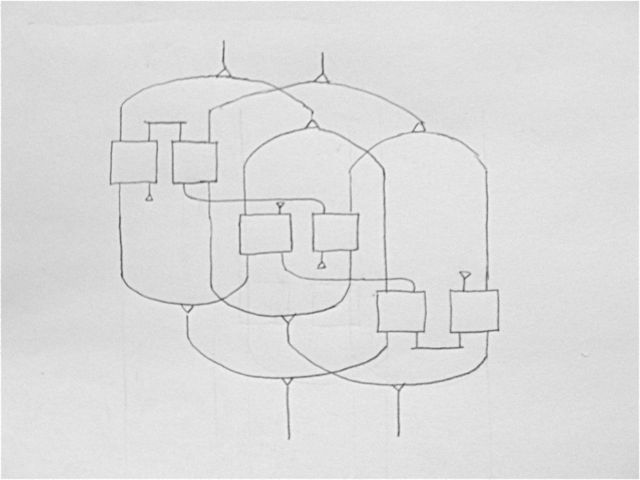
\includegraphics[scale=0.5]{./threeboxes.png}
\end{center}

\end{proof}



% \iflmcs\else\let\oldurl\url\renewcommand{\url}[1]{\hfill\break\oldurl{#1}}\fi
%
% \bibliographystyle{alpha}
% \bibliography{di-biblio}

\end{document}